\chapter[Referencial Teórico]{Referencial Teórico}

Antes de detalhar o projeto a ser desenvolvido será apresentado um resumo breve sobre a arquitetura dos microcontroladores bem como informações sobre o uso deles.   Além disso será apresentada uma visão geral do mercado com relação a disponibilidade de microcontroladores, placas de desenvolvimento, módulos e componentes.

\section[Microcontroladores]{Microcontroladores}

Como base para o trabalho é necessário conhecer o funcionamento de um microcontrolador, \citeonline{Basics2008} consegue detalhar muito bem suas características e as mais relevantes podem ser encontradas a seguir.

Em \citeonline{DinisGaspar2010, DinisGaspar2010a,DinisGaspar2010b} também é possível encontrar informações muito claras a respeito especificamente da MSP430, família de microcontroladores que será melhor detalhada posteriormente.

\subsection{Hardware dos Microcontroladores}

De maneira prática, um microcontrolador é um pequeno computador capaz de executar instruções pré-programadas, entretanto é construído em apenas um circuito integrado que contém todos os subsistemas necessários para seu funcionamento, dentre eles a unidade de processamento central (CPU, sigla para Central Processing Unit), a memória e os periféricos programáveis de entrada e saída.

\begin{figure}[h!]
  \centering
  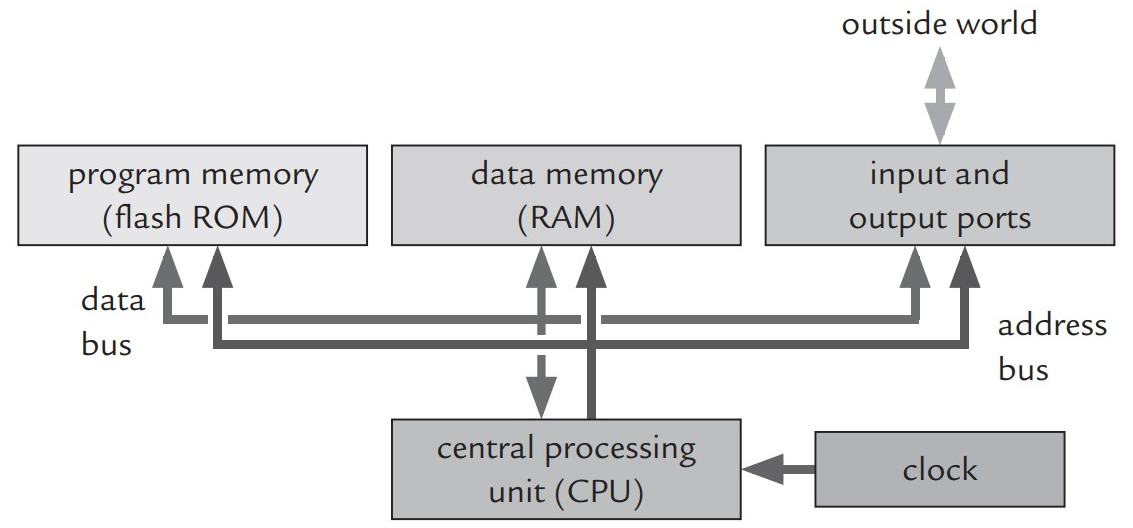
\includegraphics[width=0.9\linewidth]{figuras/componentes-microcontrolador.png}
  \caption{Subsistemas básicos de um microcontrolador} Fonte: \cite{Basics2008}
  \label{fig:arq_micro}
\end{figure}

\subsubsection{Unidade de processamento central}

Responsável por executar efetivamente as operações, este subsistema conta com os seguintes componentes:

\textbf{Unidade lógica aritmética (ULA)}: Realiza os cálculos necessários nas operações, embora cada microntrolador possa apresentar diferentes conjuntos de instruções, operações básicas como soma, subtração, AND, OR e deslocamento de bits são alguns dos exemplos de funções que as ALUs podem fazer.

\textbf{Registadores}: Além de fornecerem espaço para as informações básicas de operação da CPU como o program counter (PC), stack poiter (SP) e status register (SR). Além disso, os registadores são responsáveis por armazenar resultados temporários.

\textbf{Outros}: Diversos outros componentes para decodificar instruções, manipular resets e interrupções.

\subsubsection{Memória}

Embora os registradores também sejam responsáveis por armazenar dados, a memória é um componente dedicado exclusivamente para essa função.

\subsubsection*{RAM}

A memória de acesso aleatório (do inglês \textit{Random Access Memory}) normalmente armazenam os dados gerados durante a execução do programa e geralmente são mais rápidas que a ROM, ser do tipo volátil é uma das suas principais características.


\subsubsection*{ROM}

A memória somente de leitura ou ROM (acrônimo em inglês de \textit{read-only memory}), responsável por armazenar o programa gerado. As memórias ROM se encaixam na categoria não-voláteis, pois são capazes de reter as informação mesmo quando a energia é removida.

Para superar a grande limitação de serem apenas para leitura, surgiram diversas opções de memórias programáveis e posteriormente regraváveis como o caso da EEPROM (Electrically-Erasable Programmable Read-Only) e da memória Flash, de longe uma das mais usadas, com funcionamento semelhante às EEPROM, têm uma grande vantagem de velocidade por trabalhar com blocos de memória e não bytes independentes \cite{harari1994flash}.

Os microcontroladores geralmente utilizam 3 tipos de memória, utilizadas para diferentes funções. Flash contento o programa em si e EEPROM com dados gerais que precisam ser salvos por longos períodos e RAM para armazenar dados temporários gerados durando a execução do programa.

\subsubsection*{Arquiteturas Von Neumann e Harvard}

Essas arquiteturas estão relacionadas a organização de memórias do sistema \cite{MeloDeOliveira2014}.

Na arquitetura de von Neumann memórias de dados e de programa compartilham o mesmo barramento, sendo uma arquitetura muito mais simples, porém tem uma desvantagem relacionada a velocidade já que tudo deve passar por um único barramento.

\begin{figure}[h!]
  \centering
  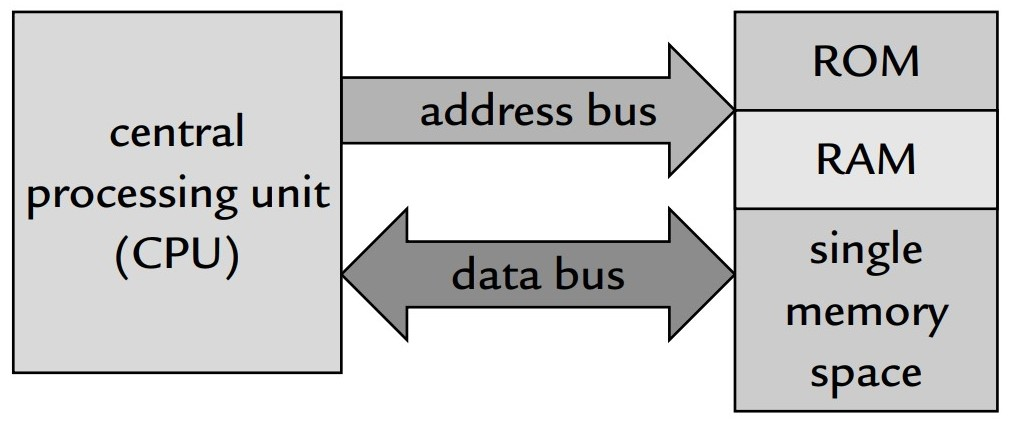
\includegraphics[width=0.5\linewidth]{figuras/vonNeumann.jpg}
  \caption{Arquitetura de von Neumann} Fonte: \cite{Basics2008}
  \label{fig:vanneumann}
\end{figure}

Já na arquitetura de Harvard essas memórias podem ser acessadas de forma simultânea, pois não compartilham o mesmo barramento, isso torna a comunicação mais rápida, em contrapartida se trata de uma arquitetura mais complexa.

\begin{figure}[h!]
  \centering
  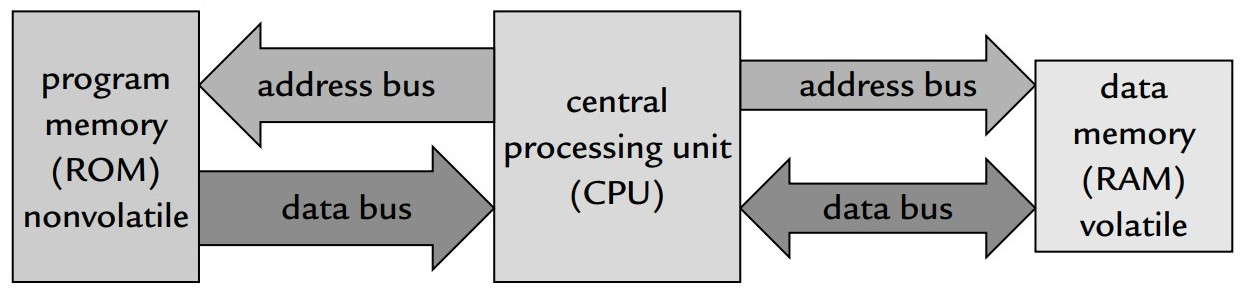
\includegraphics[width=0.8\linewidth]{figuras/harvard.jpg}
  \caption{Arquitetura de Harvard} Fonte: \cite{Basics2008}
  \label{fig:harvard}
\end{figure}

\subsubsection*{Barramentos de endereço e dados}

A comunicação entre todos os componentes acontece a todo momento e a velocidades muitos altas, para tornar isso possível é necessário criar essas ligações, que geralmente são separadas entre barramento de endereços, carregando informações a respeito do dispositivo com o qual está se comunicando e barramento de dados, onde efetivamente se trafegam os dados entre dispositivos.

\subsubsection{Entradas e Saídas}

Ponto fundamental dos microcontroladores, estes componentes são responsáveis por fornecer comunicação com o mundo exterior, podendo se dar de maneira digital e/ou analógica em alguns microcontroladores. Este componente é conhecido como GPIO, sigla para \textit{General Purpose Input/Output}.

Os microntroladores de forma geral trazem uma série de funcionalidades \cite{Johnston2018} para os GPIO buscando torná-los versáteis e robustos a diversas aplicações.

\subsubsection*{Comparadores com histerese}

Os comparadores com histerese, Schmitt-trigger, estão presentes em todas as portas GPIO de muitos microcontroladores e na maioria das vezes é utilizado com padrão ao utilizar um porta como entrada, seu papel é decidir se a entrada está em nível alto ou baixo. Ele conta dois limiares diferentes para a mudança de estado, o que torna a entrada mais imune a ruídos.

\subsubsection*{Resistores pull-up e pull-down}

Em grande parte das aplicações não é interessante deixar uma entrada com uma tensão flutuante, a utilização de resistores de pull-up, conectando sinal à alimentação, e pull-down, sinal ao terra, é muito comum, e por isso alguns microcontroladores já trazem essa funcionalidade internamente.

\begin{figure}[h!]
  \centering
  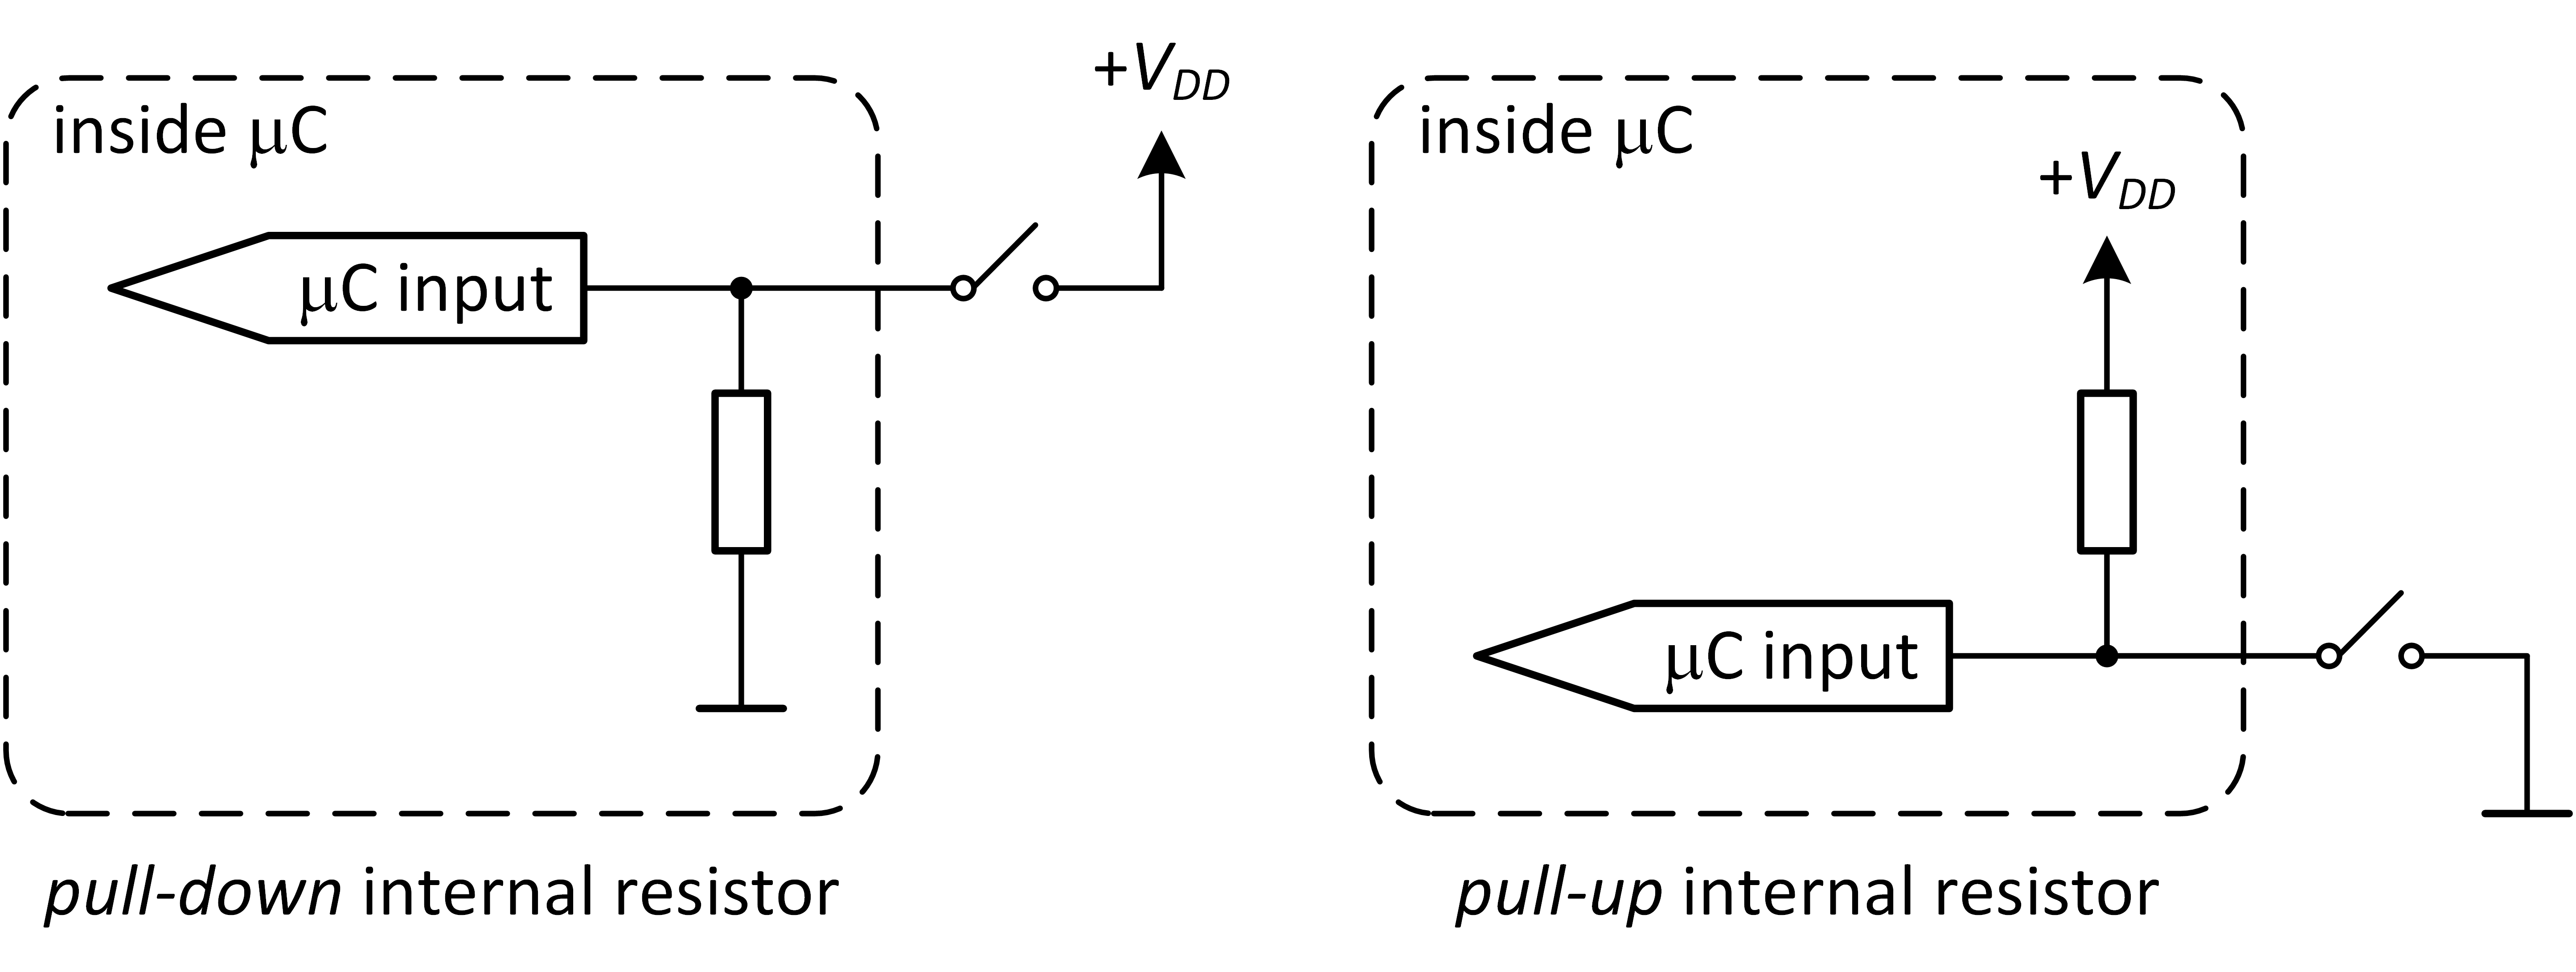
\includegraphics[width=0.8\linewidth]{figuras/input.png}
  \caption{Tipos de entrada} Fonte: \cite{DigitalIO}
  \label{fig:input}
\end{figure}

\subsubsection*{Detecção de borda}

Além de ser possível identificar o nível lógico da entrada, grande parte dos microcontroladores também são capazes de detectar a variação desse sinal, nível lógico 0 para 1, borda de subida, e vice-versa, borda de descida.

\subsubsection*{Saída de coletor aberto, dreno aberto e push-pull}

Os microcontroladores podem ter diversas formas de controlar sua saída, geralmente são utilizados transitores ou MOSFETs em dois tipos de configuração.

No caso da push-pull a topologia utilizada permite a saída ter dois valores de tensão, 0V ou VDD (figura \ref{fig:output}), já para saídas do tipo coletor aberto (em transitores) ou dreno aberto (em MOSFETs) a saída pode assumir 0V ou alta impedância.

\begin{figure}[h!]
  \centering
  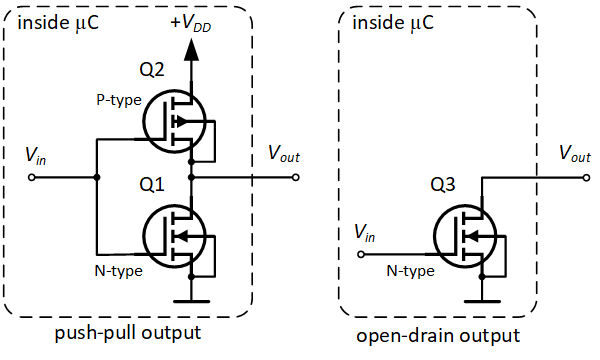
\includegraphics[width=0.7\linewidth]{figuras/output.png}
  \caption{Tipos de saída} Fonte: \cite{DigitalIO}
  \label{fig:output}
\end{figure}

\subsubsection{Interrupções}

Geralmente gerado por hardware, embora possa ser iniciado por software, as interrupções indicam que ocorreu um evento que precisa de uma resposta urgente. O valor de leitura de uma entrada é modificado, por exemplo, e é necessário verificar seu estado. O processador interrompe o que estava fazendo, armazena informações suficiente ( \textit{program counter} e \textit{status register}) para que ele continue mais tarde e executa uma rotina de serviço de interrupção (ISR). Ele retorna à sua atividade anterior quando o ISR foi concluído. Assim, um ISR é algo como uma sub-rotina chamada por hardware e não por software \cite{Basics2008}.

\subsubsection{Sinal de Relógio}

Praticamente todos os sistemas digitais necessitam de um sinal de relógio para funcionarem, são conhecidos como pelo termo em inglês \textit{clock}. É neste componente onde isso é gerado, pode ser obtido através de um cristal ou fontes externa. Atualmente os microcontroladores são capazes de gerar e trabalhar com uma faixa relativamente grande de frequências.

\subsubsection{Temporizadores}

Como uma extensão dos clocks, os temporizadores são muito versáteis e necessários para diversas funções do microcontrolador, como por exemplo gerar sinais de clock para outros periféricos do chip, calcular intervalos de tempo ou medir período de sinais.

\subsubsection*{Contadores}

Um contador é um dispositivo que armazena  o número de vezes que um evento ou processo específico ocorreu, geralmente em relação a um sinal de relógio. Os contadores são divididos em duas categorias, os síncronos e assíncronos e embora possam apresentar diversas topologias um circuito  contador é geralmente construído com flip-flops conectados em cascata \cite{Floyd2007}.

\subsubsection*{Watchdog Timer}

Como ferramenta de segurança esse contador é responsável por resetar o microcontrolador caso o programa entre em um loop infinito.

\subsubsection{Interfaces de comunicação}

Ampliando a função de Entradas e Saídas, as interfaces de comunicação fornecem protocolos próprios para a transmissão de dados buscando sempre transmitir de maneira rápida e com baixas taxas de perda, dentre as mais comuns presentes nos microcontroladores temos como exemplo a Serial Peripheral Interface (SPI), Inter-Integrated Circuit (I2C) e Universal Asynchronous Receiver/Transmitter (UART).

\subsubsection{Conversores}
\label{sec:conversores}

Dados do mundo exterior são essencialmente analógicos, e para tornar a interação com circuitos que trabalham dessa maneira os conversores são peça indispensável. Essa conversão pode acontecer em dois sentidos, convertendo um sinal analógico em digital (A/D) e vice-versa (D/A).

Em ambos os casos existem duas grandezas de extrema importância, a resolução e a frequência de amostragem do sinal. A resolução está ligada diretamente ao erro de quantização e consequentemente à relação sinal-ruído da conversão. Já a frequência de amostragem está relacionada à velocidade com que o conversor pega amostras do sinal analógico.

Existem inúmeras topologias que tentam otimizar essas características de desempenho com simplicidade do circuito.

\subsubsection*{Comparadores}

Utilizados em algumas topologias de conversores A/D, os comparadores são dispositivos que comparam duas tensões ou correntes e indicam qual delas é maior. Podem ser utilizados como detectores de passagem por zero e em alguns casos podem ser configurados para funcionarem como Schmitt trigger, no MAX971 \cite{Integrated2003} por exemplo.

\subsection{Linguagens de Programação}

A programação de um microcontrolador percorre diversos níveis de forma a converter o código escrito para a linguagem de máquina.

\subsubsection*{Linguagem de Máquina}

A linguagem de máquina consiste em um código binário que o processador consegue entender. No início da computação a programação era feita dessa forma, mas hoje em dia não é mais necessário trabalhar nessa linguagem de baixo-nível.

\subsubsection*{Linguagem de Montagem}

Um nível um pouco, só um pouco, acima da linguagem de máquina temos a linguagem de montagem, comumente conhecida como Assembly, ela traduz o código binário para algumas palavras conhecidas como mnemónicos.

Uma grande desvantagem é que essa tradução de código binário depende diretamente do processador, ou seja, cada tipo de processador tem um dicionário de palavras único. Em compensação ao utilizar o Assembly consegue-se ter mais controle sobre a eficiência do código e, além disso, é possível ver exatamente o comportamento de processador no processo de debug.

\subsubsection*{Linguagem C}

Uma das linguagem de programação mais usadas para a programação de microcontroladores, por ser uma linguagem de alto-nível é possível criar lógicas complexas sem muito trabalho e sem a necessidade de conhecer todo conjunto de instruções do processador.
A desvantagem fica por conta da compilação que pode não ser a mais eficiência, embora atualmente os compiladores estão cada vez melhores e trabalham muito bem esse ponto.

\subsection{Programando um Microcontrolador}

Normalmente é possível programar um microcontrolador em qualquer uma das linguagens citadas acima, respeitando o conjunto de instruções de cada modelo.

Para efetivamente programar o chip normalmente é utilizado um ambiente de desenvolvimento integrado (IDE, do inglês Integrated Development Environment), existem diversos disponíveis, entretanto a maioria das fabricantes têm seu próprio ambiente como o Code Compose Studio da Texas Instruments e MPLAB X da Microchip.

No ambiente educacional existem também outras IDE que são muito utilzadas devido a sua maior simplicidade, como o Arduíno IDE e Energia, plataformas de código aberto com suporte à algumas famílias de microcontroladores.

\subsection{Aplicações}

Microcontroladores são utilizados em praticamente qualquer dispositivo automatizado, isso pode incluir sistemas de controle de automóvel, dispositivos médicos implantáveis, controles remoto, máquinas de escritório, eletrodomésticos, ferramentas elétricas, brinquedos, entre muitos outros.

São diversos pontos que contribuem para sua grande utilização, mas o que mais pode-se destacar é seu custo e consumo de energia. Além disso, vantagens como facilidade de programação e arquitetura simplificada tornam os microcotroladores uma das melhores opções para prototipagem de projetos.

\subsection{Uso da Educação}

Se tratando especificamente de kits de desenvolvimento voltados para educação, trabalhos como \citeonline{Martin-Ramos2017}, \citeonline{Deaky2011}, \citeonline{Nunnally1996} e \citeonline{BittencourtdaSilva2015} conseguem destacar muito bem a importâncias deles no aprendizado em geral, não só no que tange ao conhecimento técnico. Embora este trabalho tenha como o foco a graduação, em \citeonline{Silveira2017} também pode se observar esse impacto no nível médio.

Ademais, existem alguns trabalhos que se posicionam de forma bem alinhada ao objetivo deste, a construção de kits e módulos próprios para auxiliar a aprendizagem no ambiente de graduação e afins como o caso de \citeonline{Dabroom2013} e \citeonline{Su2013}.

\section{Opções do Mercado}

É muito importante mapear algumas opções de placas, módulos, componentes entre outros visando ter um olhar geral sobre o que é possível encontrar no mercado brasileiro, já que além de suprir as necessidades do aprendizado de microcontroladores, este trabalho também tem como objetivo construir shields acessíveis para os alunos.

\subsection{Microcontroladores e Placas}

Quando se trata do desenvolvimento de produtos, a utilização de microcontroladores não é feita usando somente o chip integrado, salvo em situações específicas, a desenvolvimento acontece sobre um kit, onde o microcontrolador é utilizado através de uma placa própria, onde a programação e o acesso ao pinos é muito mais fácil.

Kits de desenvolvimento já são muito comuns no mercado, são utilizados tanto no ensino quando em empresas para testes de novos produtos.

"[O Arduino, por exemplo,] se tornou um produto extremamente bem-sucedido junto a fabricantes, estudantes e artitas, devido à sua facilidade de uso e durabilidade" \cite{Monk2013}. 

Outra placa que vem se destacando muito no mercado é a ESP32, com uma CPU de dois núcleos de 32 bits e integrada a módulos Wifi e Bluetooh é sem dúvida a placa com melhor custo-benefício do mercado.

Em contrapartida, temos a família de placas MSP430, com CPU de 16 bits apresentam um meio termo em as outra opções , mesmo não disponível no mercado brasileiro é muito utilizado no ambiente acadêmico e de empresas por se destacar muito no quesito consumo de energia.

Na tabela \ref{tab:placas} encontra-se algumas das principais características das placas de desenvolvimento.

\begin{table}[h!]
\centering
\resizebox{\textwidth}{!}{%
\begin{tabular}{|c|c|c|c|c|c|}
\hline
	 & CPU                     & RAM & Flash & GPIO & Preço  \\ \hline
Arduino Uno              & ATmega328 8-bit         & 2 KB        & 32 KB         & 20                        & $\sim$R\$ 50,00 \\ \hline
Arduino Mega             & ATmega2560 8-bit        & 8 KB        & 256 KB        & 70                        & $\sim$R\$ 90,00 \\ \hline
MSP-EXP430G2ET           & MSP430G2553 16-bit      & 512 B       & 16KB          & 16                        & \$ 10,00        \\ \hline
MSP-EXP430F5529LP        & MSP430F5529 16-bit      & 8 KB         & 128KB         & 32                        & \$ 13,00        \\ \hline
ESP32                    & Xtensa Dual-Core 32-bit & 520 KB      & 4 MB          & 25                        & $\sim$R\$ 70,00 \\ \hline
\end{tabular}%
}
\caption{Principais placas de desenvolvimento}
\label{tab:placas}
\end{table}

Todas as placas contam com suporte a comunicação serial e entradas analógicas com conversores A/D de 10 bits ou mais.

\subsection{Shields}

Para expandir as funcionalidades surgiram as placas conhecidas como shields, que por sua vez incorporam diferentes tipos de módulos para facilitar ainda mais o desenvolvimento e testes de protótipos.

No mercado brasileiro as shields ainda são restritas uma pequena variedade de módulos e, como maior impedimento, desenvolvidas para os kits com base em Arduino, modelos UNO e MEGA.

O uso desses shields é extremamente simples, bastando encaixá-los sobre o kit de desenvolvimento.

\begin{figure}[h!]
\centering
  \begin{subfigure}[b]{0.5\textwidth}
  \centering
    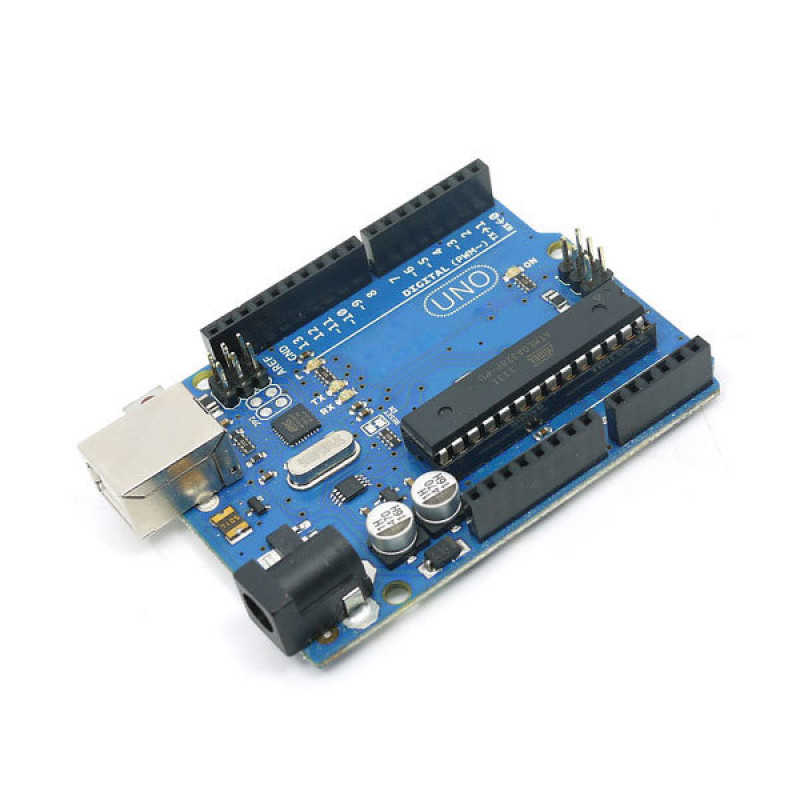
\includegraphics[width=\textwidth]{figuras/arduino_uno.jpg}
    \caption{Arduino Uno} Fonte: \cite{bib_uno}
    \label{fig:arduino}
  \end{subfigure}
  %
  \begin{subfigure}[b]{0.4\textwidth}
  \centering
    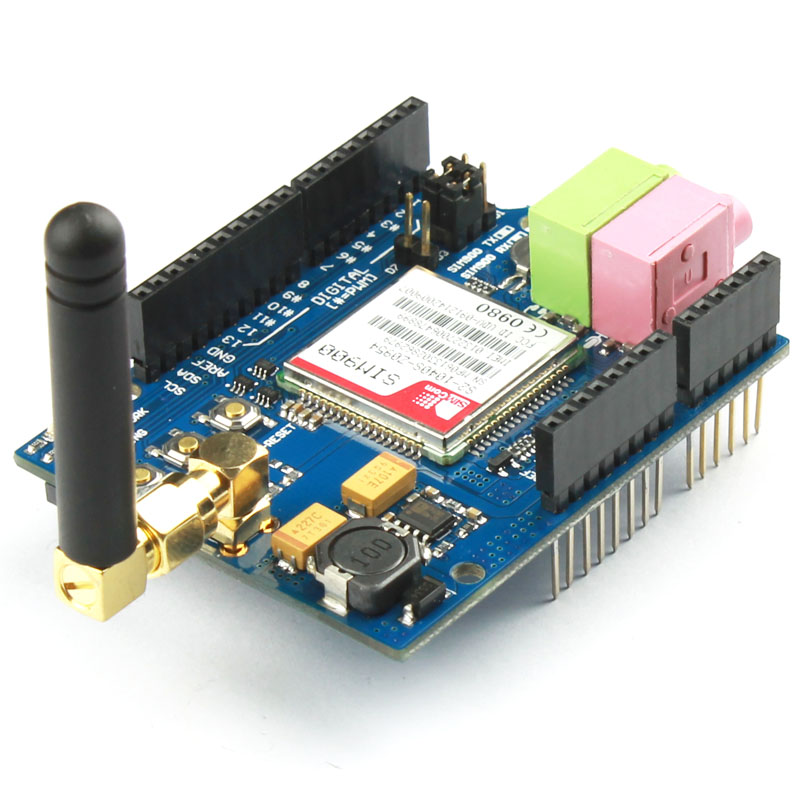
\includegraphics[width=\textwidth]{figuras/shield_gsm.jpg}
    \caption{Shield GSM} Fonte: \cite{bib_gsm}
    \label{fig:shield_gsm}
  \end{subfigure}
  \caption{Kit e shield comum no mercado brasileiro.}
\end{figure}

\subsubsection{BoosterPack}

Os kits de desenvolvimento disponibilizados pela Texas Instruments têm como foco não só agilizar o desenvolvimento mas também auxiliar na educação, por isso além das LaunchPads a empresa conta com os \textit{BoosterPack plug-in modules}.

Os BoosterPack são módulo que podem ser integrados aos kits de desenvolvimento para fornecer recursos e funcionalidades adicionais para fornecer recursos e funcionalidades adicionais, incluindo recursos de detecção de toque \cite{TexasInstruments}, infravermelho \cite{TexasInstrumentsa}  e bateria \cite{TexasInstrumentsb}.

Além dos módulos já citados, a Texas Instruments também desenvolveu um BoosterPack com foco educacional, o \textit{Educational BoosterPack MKII} \cite{TexasInstrumentsc}, ele conta com diversos módulos e um suporte especial através do \textit{Energia}, ambiente de desenvolvimento de código aberto feito pela comunidade.

È possível encontrar outros kits que seguem a linha de BoosterPacks criados por grupos e/ou desenvolvedores \cite{43oh} que serviram de inspiração para este trabalho já que todos os kits e módulos citados são extremamente escassos no Brasil, e seu custo de importação muitas vezes pode inviabilizar sua utilização.

\subsection{Módulos e componentes}

Como o objetivo deste trabalho é construir novas shields,  é necessário conhecer opções de módulos e componentes disponíveis no mercado para tornar a etapa de fabricação viável.

\subsubsection{Interfaces}

\subsubsection*{Leds}

Um dos componentes mais clássicos da eletrônica e utilizado em quase todos os projetos, também tem papel fundamental no aprendizado, sendo um dos primeiros componentes utilizados durante as aulas.

Basicamente podemos pensar em duas categorias básica, os LEDs monocromáticos e os RGB que podem ter sua cor controlada digitalmente.

Aqui características como consumo e tensão de operação são os pontos críticos. Na tabela \ref{tab:leds} é possível observar algumas diferenças fundamentais.

\begin{table}[h!]
\centering
\begin{tabular}{|c|c|l|l|}
\hline
      			& Tensão 		& Corrente& Dimensões 		\\ \hline
LED RGB 		& min. 3.2 V 	&	30 mA & 5 x 5 x 10 mm \\ \hline
LED Difuso 		& min. 2 V  	&   20 mA & 5 x 5 x 10 mm \\ \hline
LED Alto Brilho & min. 2 V 		&	30 mA & 5 x 5 x 10 mm \\ \hline
\end{tabular}
\caption{Comparação LEDs}
\label{tab:leds}
\end{table}

\begin{figure}[h!]
\centering
  \begin{subfigure}[b]{0.3\textwidth}
  \centering
    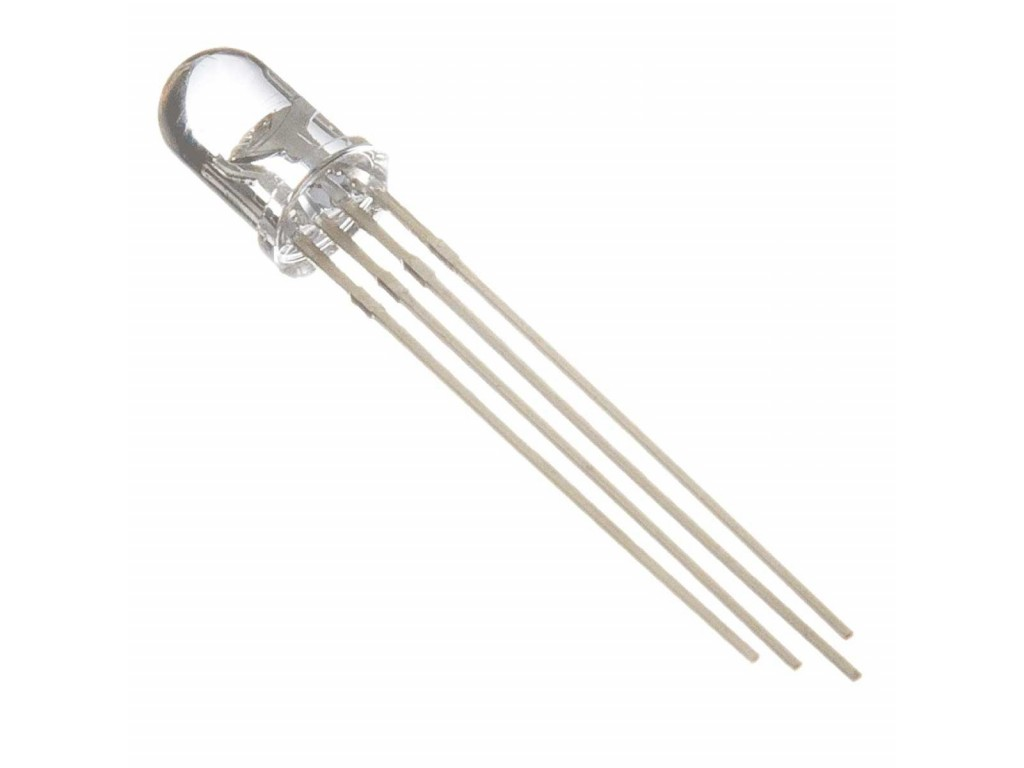
\includegraphics[width=\textwidth]{figuras/led_rgb.jpg}
    \caption{LED RGB} Fonte: \cite{Elcoteam2019}
    \label{fig:led_rgb}
  \end{subfigure}
  %
  \begin{subfigure}[b]{0.22\textwidth}
  \centering
    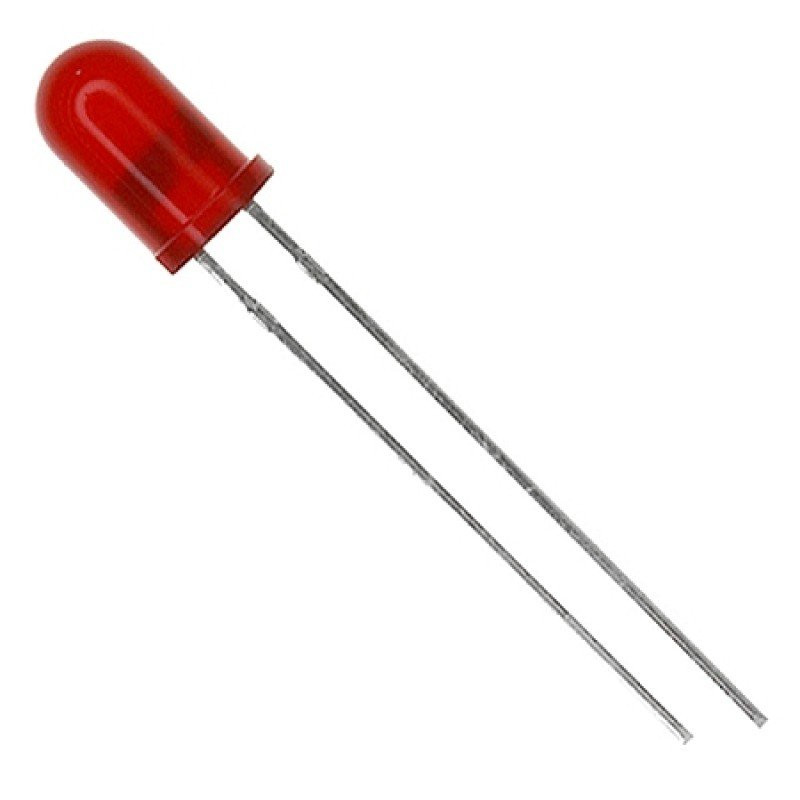
\includegraphics[width=\textwidth]{figuras/led_difuso.jpg}
    \caption{LED Difuso} Fonte: \cite{BaudaEletronica2019}
    \label{fig:led_difuso}
  \end{subfigure}
  %
  \begin{subfigure}[b]{0.3\textwidth}
  \centering
    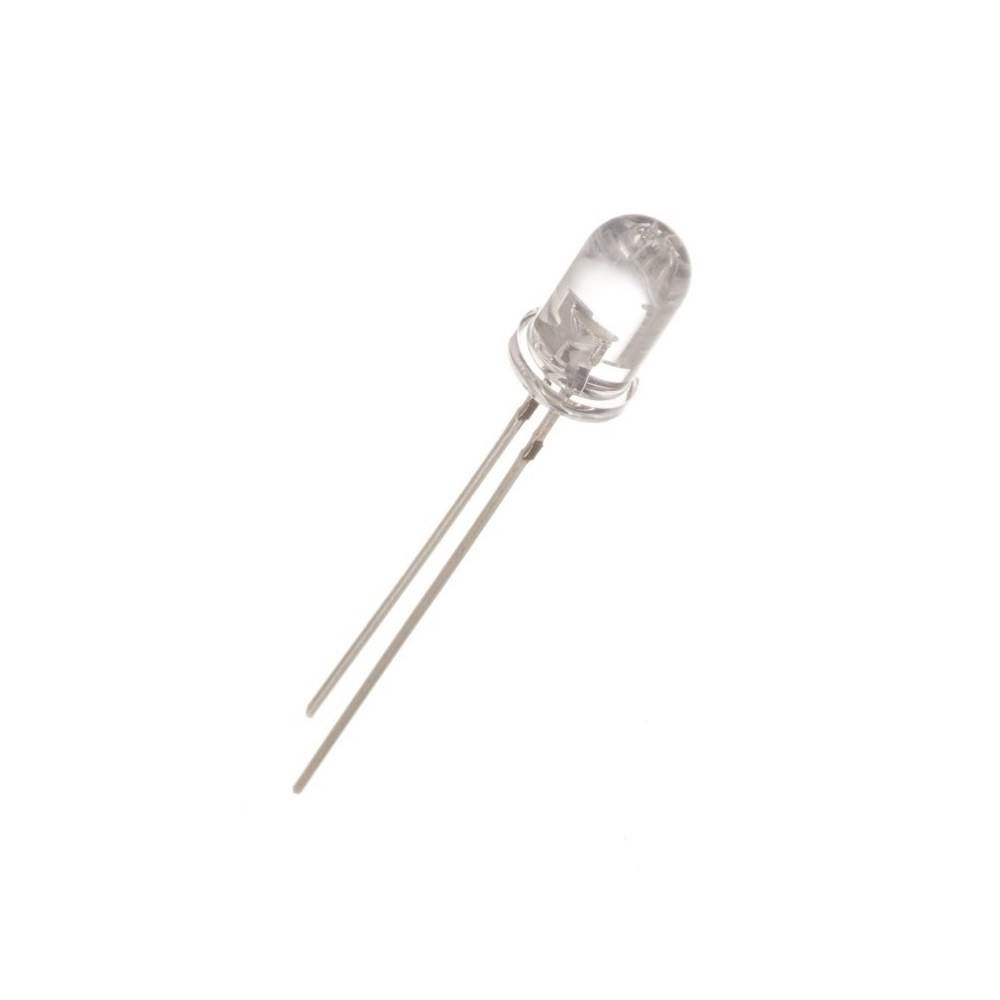
\includegraphics[width=\textwidth]{figuras/led_alto_brilho.jpg}
    \caption{LED Alto Brilho} Fonte: \cite{CurtoCircuito2019}
    \label{fig:led_alto_brilho}
  \end{subfigure}
  \caption{Opções de LEDs}
\end{figure}

\subsubsection*{Display}

Displays de forma geral facilitam muito a visualização de informações, no mercado brasileiro existem algumas opções sendo 3 delas (figura \ref{fig:displays}) muito utilizadas em projetos.

\begin{table}[h!]
\centering
\begin{tabular}{|c|c|c|l|l|l|}
\hline
                & Tensão	& Corrente	& Tipo de Comunicação	& Dimensões \\ \hline
Display OLED    & 3-5.5 V  &  25 mA    &          I2C			&          30 x 27 x 4 mm \\ \hline
Display Nokia 5110 &  3.3-5.5 V & 50 mA &		 SPI			&          
45 x 43 x 5 mm \\ \hline
Display 16x2  	&	4.5-5.5 V	&	140 mA	&  Paralela 8 bits	& 80 x 36 x 12 mm \\ \hline
\end{tabular}
\caption{Comparação Displays}
\label{tab:displays}
\end{table}


\begin{figure}[h!]
\centering
  \begin{subfigure}[b]{0.3\textwidth}
  \centering
    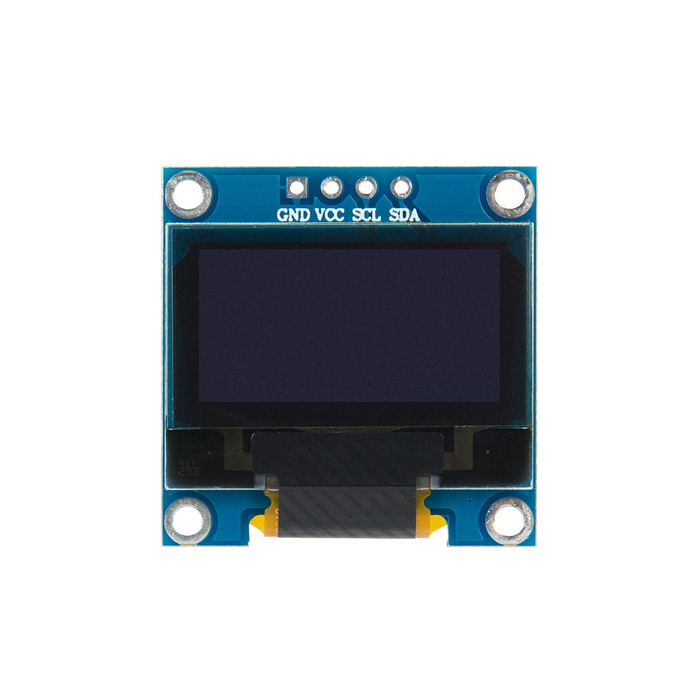
\includegraphics[width=\textwidth]{figuras/display_oled.jpg}
    \caption{Display OLED} Fonte: \cite{FilipeFlop2019}
    \label{fig:display_oled}
  \end{subfigure}
  %
  \begin{subfigure}[b]{0.3\textwidth}
  \centering
    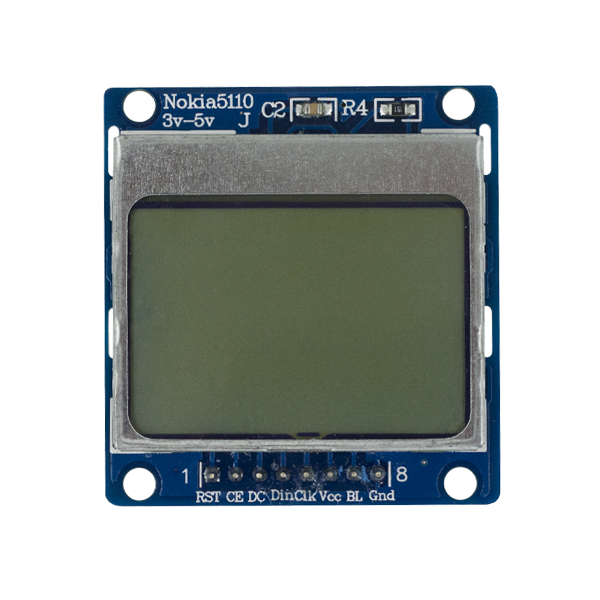
\includegraphics[width=\textwidth]{figuras/display_nokia.png}
    \caption{Display Nokia 5110} Fonte: \cite{FilipeFlop2019a}
    \label{fig:display_nokia}
  \end{subfigure}
  %
  \begin{subfigure}[b]{0.3\textwidth}
  \centering
    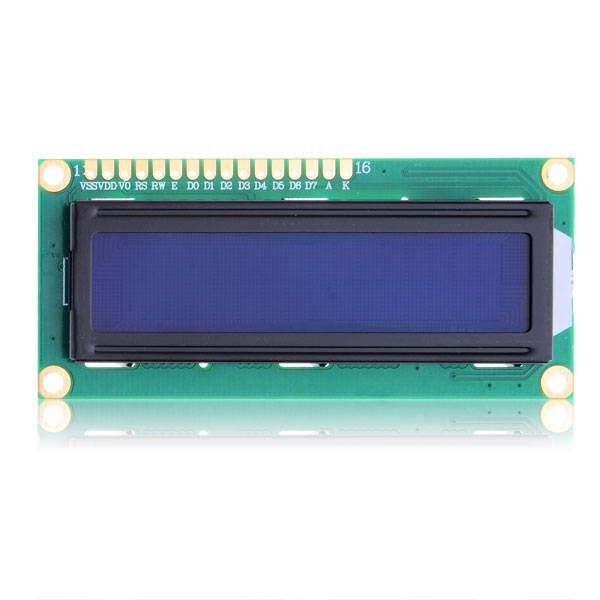
\includegraphics[width=\textwidth]{figuras/display_16x2.jpg}
    \caption{Display 16x2} Fonte: \cite{FilipeFlop}
    \label{fig:display_16x2}
  \end{subfigure}
  \caption{Opções de displays}
  \label{fig:displays}
\end{figure}

\paragraph*{Display 7 Segmentos}

Também na categoria de displays, o display de 7 segmentos serve com um meio termo entre os LEDs e Displays, sua utilização é muito vantajosa quando se trata de exibição de números, já que sua é muito mais simples do que um display comum e bem mais elegante do que a utilização de LEDs.

Essencialmente existe apenas um modelo de display de 7 segmentos, bastando utilizar componentes integrados extras para facilitar ainda mais sua utilização.

\begin{figure}[h!]
  \centering
    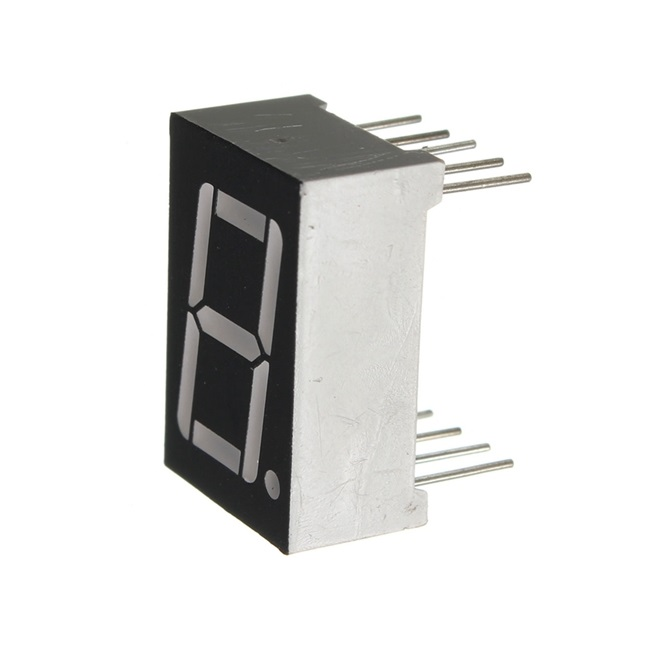
\includegraphics[width=.3\textwidth]{figuras/7seg.jpg}
    \caption{Display 7 Segmentos} Fonte: \cite{FilipeFlop2019b}
    \label{fig:7seg}
\end{figure}

Apesar de versátil o display de 7 segmentos tem uma grande limitação que pode tornar sua utilização inviável, o número de conexões. Tal limitação pode ser resolvida com módulos um pouco mais complexos que utilizam da comunicação I2C por exemplo.

\subsubsection{Sensores}

Converter informação do ambiente em sinais elétricos é o princípio de funcionamento de um sensor, normalmente são a base de qualquer projeto.

Existem uma infinidade de sensores capazes de medir qualquer estímulo do ambiente, entretanto alguns deles apresentam certa versatilidade que pode ser muito útil para um kit de desenvolvimento.

\subsubsection*{Temperatura}

Quando se pensa em sensores com certeza este é o primeiro a vir a mente, monitorar temperatura é só um exemplo da usabilidade desse sensor.

Novamente temos uma grande quantidade de modelos e aqui não temos muitas restrições, e por isso a caraterística mais importante para a escolha desse sensor deve ser sua forma de funcionamento, com ou sem contato.

Um dos modelos mais comuns no mercado é o DHT11 \cite{AOSONG2010}, que além de medir temperatura também conta com um sensor de umidade.

\begin{table}[h!]
\centering
\begin{tabular}{|c|c|}
\hline
\multicolumn{2}{|c|}{DTH11}              \\ \hline
Tensão                  & 3-5.5 V        \\ \hline
Corrente                & 100-500 uA     \\ \hline
Faixa de Temperatura    & 0-50 °C        \\ \hline
Precisão de Temperatura & ± 2 °C         \\ \hline
Faixa de Umidade        & 20-90 \%       \\ \hline
Precisão de Umidade     & ± 5 \%         \\ \hline
Dimensões               & 18 x 12 x 5 mm \\ \hline
\end{tabular}
\caption{Características do Sensor de Temperatura e Umidade}
\label{tab:temp}
\end{table}

\subsubsection*{Acelerômetro}
\label{sec:acel}

O acelerômetro é outro sensor extremamente versátil, sua utilização é relacionada a qualquer tipo de projeto que trate de movimentação.

Existem basicamente 3 modelos disponíveis no mercado brasileiro o \textit{MMA7361} \cite{FreescaleSemiconductor2011}, o \textit{ADXL335} \cite{AnalogDevices2009} e o \textit{MPU-6050} \cite{InvenSence2013}, ambos com características semelhantes e comunicação serial, entretanto o último conta com um ponto de destaque, o mesmo circuito integrado contém um giroscópio e que o torna muito mais vantajoso.

\begin{table}[h!]
\centering
\begin{tabular}{|c|c|}
\hline
\multicolumn{2}{|c|}{MPU-6050}                  \\ \hline
Tensão               & 3-5 V                    \\ \hline
Conversor A/D        & 16 bits                  \\ \hline
Comunicação          & I2C                      \\ \hline
Escalas Giroscópio   & ±250, 500, 1000, 2000 °/s \\ \hline
Escalas Acelerômetro & ±2, ±4, ±8, ±16g         \\ \hline
Dimensões            & 2 x 1,6 x 0,1mm          \\ \hline
\end{tabular}
\caption{Características do Acelerômetro}
\label{tab:acel}
\end{table}

\subsubsection*{Luminosidade}

Medir luminosidade é algo simples e restrito a um pequeno número de projetos, entretanto é algo de fácil implementação e favorece o entendimento sobre utilização do conversor A/D.

O sensor mais simples e que cumpre muito bem sua função é o LDR \cite{Technologies2008}, as opções de 5 e 3 mm devem ser consideradas.

\paragraph*{Infravermelho}

Como uma extensão dos sensores de luminosidade, o sensor infravermelho é capaz de detectar o espectro infravermelho de luz, na prática é uma luz invisível para o olho humano mas que é muito utilizado em controles remoto por exemplo.

Da mesmo forma que o LDR, sua aplicação é limitada, mas se tratando de aprendizado, este módulo pode trazer uma nova perspectiva, já que seu funcionamento se baseia em pulsos de sinal.

O módulo encontrado no mercado é o \textit{TSOP4838} \cite{Semiconductors2018}.

\begin{table}[h!]
\centering
\begin{tabular}{|c|c|}
\hline
\multicolumn{2}{|c|}{TSOP4838} \\ \hline
Tensão             & 2.7-5.5 V \\ \hline
Frequência         & 38 kHz    \\ \hline
Ângulo de detecção & 45°       \\ \hline
Dimensões          & 30 x 5 mm \\ \hline
\end{tabular}
\caption{Características do Receptor Infravermelho}
\label{tab:infra}
\end{table}

\subsubsection*{Botões}

Mais um dos componentes que são praticamente indispensáveis em qualquer projetos, os botões tem um funcionamento simples e são utilizados para iteração do usuário com o projeto. 

Os botões e chaves de maneira geral podem ser classificados de acordo com duas caracteríticas, número de circuitos que pode controlar ao mesmo tempo (polos) e quanto ao seu acionamento (único ou duplo).

Para o número de circuitos temos as siglas:

\begin{itemize}
	\item SP, 1 polo;
	\item DP, 2 polos;
	\item 3P, 3 polos;
	\item 4P, 4 polos.
\end{itemize}

Com relação o tipo de funcionamento temos:

\begin{itemize}
	\item ST para acionamento único;
	\item DT para acionamento duplo.
\end{itemize}

Além de seu funcionamento, o formato do botão também deve ser um fator relevante na escolha.

\subsubsection{Atuadores}

Atuadores é o nome dado a componentes que produzem movimento através de comandos elétrico e/ou mecânicos.

\subsubsection*{Relés}

Comumente conhecido com relé, os interruptores eletromecânicos são, de maneira prática, componentes capazes de controlar eletronicamente circuitos de alta tensão.

Aqui temos poucas opções, principalmente porque seu funcionamento é extremamente simples, a grande diferença encontrada entre os modelos do mercado é com relação a sua tensão de ativação.

\begin{figure}[h!]
  \centering
    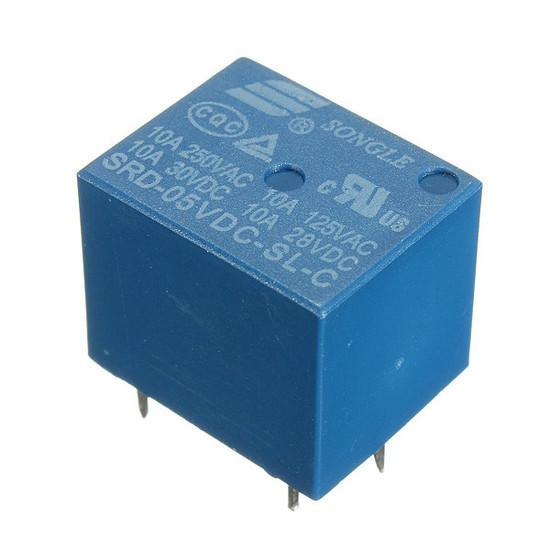
\includegraphics[width=.3\textwidth]{figuras/rele.jpg}
    \caption{Relé} Fonte: \cite{FilipeFlop2019g}
    \label{fig:rele}
\end{figure}

\subsubsection*{Motores de Passo}

A uso de motores de passo se faz com a utilização de controladores, conhecidos como drivers, capazes de fornecer a potência necessária para esses motores, é possível projetar esse tipo de circuito, entretanto isso foge do escopo deste trabalho, portanto neste projeto será utilizado módulos prontos capazes de executar tal função. Novamente existem diversas opções, mas temos uma grande restrição quando se trata desses drivers, o seu tamanho e dissipação de potência.

Para não esbarrar em nenhuma dessas restrições os módulos não serão de grande capacidade, controlando apenas motores de passo de pequeno porte. Considerando essa restrições temos as 3  \cite{STMicroelectronics2002,TexasInstruments214,MicroSystems2014} opções descritas na tabela \ref{tab:drivers}

\begin{table}[h!]
\centering
\begin{tabular}{|c|c|c|}
\hline
        & Tensão de Alimentação & Corrente Máxima de Saída \\ \hline
ULN2003 & 5-12 V                & 500 mA                   \\ \hline
DRV8825 & 8.2-45 V              & 1.5 A                    \\ \hline
A4988   & 8-35 V                & 1 A                      \\ \hline
\end{tabular}
\caption{Comparação de drivers para motores de passo.}
\label{tab:drivers}
\end{table}


\subsubsection*{Motores de DC}

Assim como para os motores de passo, os motores de corrente contínua (DC) também necessitam de um driver para fornecer potência, entretanto temos poucas opções disponíveis no mercado, sendo o L298N \cite{STMicroelectronics2013} o mais comum.

\begin{table}[h!]
\centering
\begin{tabular}{|c|c|}
\hline
\multicolumn{2}{|c|}{L298N}          \\ \hline
Tensão de Alimentação     & 7 - 35 V \\ \hline
Canais                    & 2        \\ \hline
Corrente máxima por canal & 2 A      \\ \hline
\end{tabular}
\caption{Especificação L298N}
\label{tab:l298n}
\end{table}

\paragraph*{Controlador Duplo}
\label{sec:duplo}

Por mais que o L298N seja o mais comum e atenda grande parte das necessidades, se trata de um módulo antigo e que se aquece bastante durante a operação, por conta disso, após algumas pesquisas, encontrou-se o TB6612FNG \cite{Toshiba2008}, driver duplo capaz de controlar tanto motores DC quanto motores de passo.

Com seu funcionamento baseado em MOSFETs, o TB6612FNG é mais eficiente e versátil além de fornecer uma boa corrente de saída.

\begin{table}[h!]
\centering
\begin{tabular}{|c|c|}
\hline
\multicolumn{2}{|c|}{TB6612FNG}                                         \\ \hline
Tensão de Alimentação           & 4.5-13.5 V		\\ \hline
Canais                          & 2          		\\ \hline
Corrente máxima por canal       & 1 A        		\\ \hline
Dimensões 						& 21 x 19 x 3.6 mm 	\\ \hline
\end{tabular}
\caption{Especificação TB6612FNG}
\label{tab:duplo}
\end{table}

\begin{figure}[h!]
  \centering
    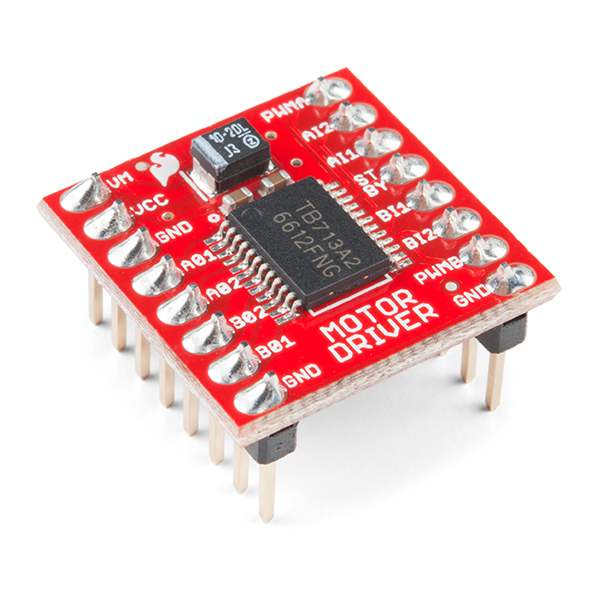
\includegraphics[width=.3\textwidth]{figuras/duplo.jpg}
    \caption{TB6612FNG} Fonte: \cite{Sparkfun2019}
    \label{fig:duplo}
\end{figure}

\subsubsection{Conectividade}

\subsubsection*{Bluetooth e Wifi}

O Bluetooh e o Wifi são duas das tecnologias de comunicação mais predominantes no dia-a-dia, por isso se tornam quase indispensáveis em grande parte dos projetos. A utilização dessa tecnologias por um microcontrolador é totalmente dependente de módulos especializados que trabalhando quase que de forma independente para se conectarem, bastando ao microcontrolador enviar comandos simples de conexão por exemplo.

Para ambas as tecnologias existem algumas opções no mercado, entretanto uma das opções abrange tanto o Bluetooh quanto o Wifi, o ESP32.

O ESP32 se trata de uma série de microcontroladores que integra o microcontrolador em si com Wifi e Bluetooh. Com alto poder de processamento e diversas interfaces de comunicação tem se tornado cada vez mais comum na prototipagem de projetos, principalmente aqueles relacionados à Internet das Coisas (IoT).

\subsubsection*{RS232}

Considerando a utilização de microcontroladores em ambientes industriais, o uso de protocolos mais robustos como o RS232 \cite{Semiconductor1998} é extremamente relevante, e para trazer esse ambiente mais próximo ao aluno, esse componente será levado em consideração na elaboração dos módulos.

\begin{figure}[h!]
  \centering
    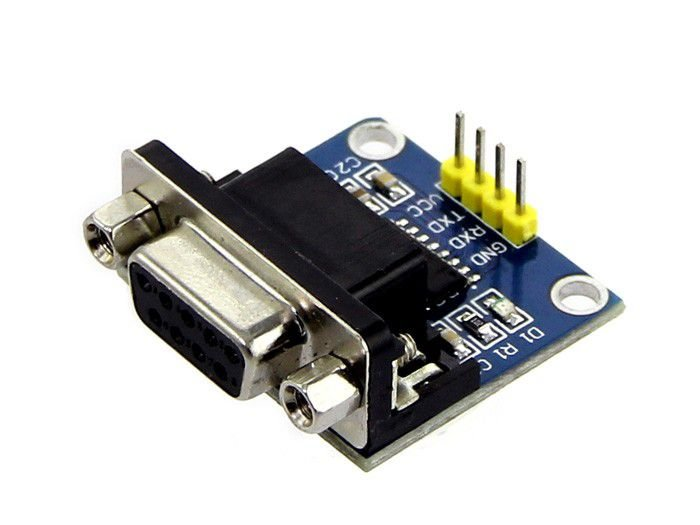
\includegraphics[width=.5\textwidth]{figuras/rs232.jpg}
    \caption{Conversor RS232} Fonte: \cite{EletroGate2019b}
    \label{fig:rs232}
\end{figure}